\section{Standard UTXO transaction}

\begin{figure}[h]
	\caption{Example of a parametric plot ($\sin (x), \cos(x), x$)}
	\centering
	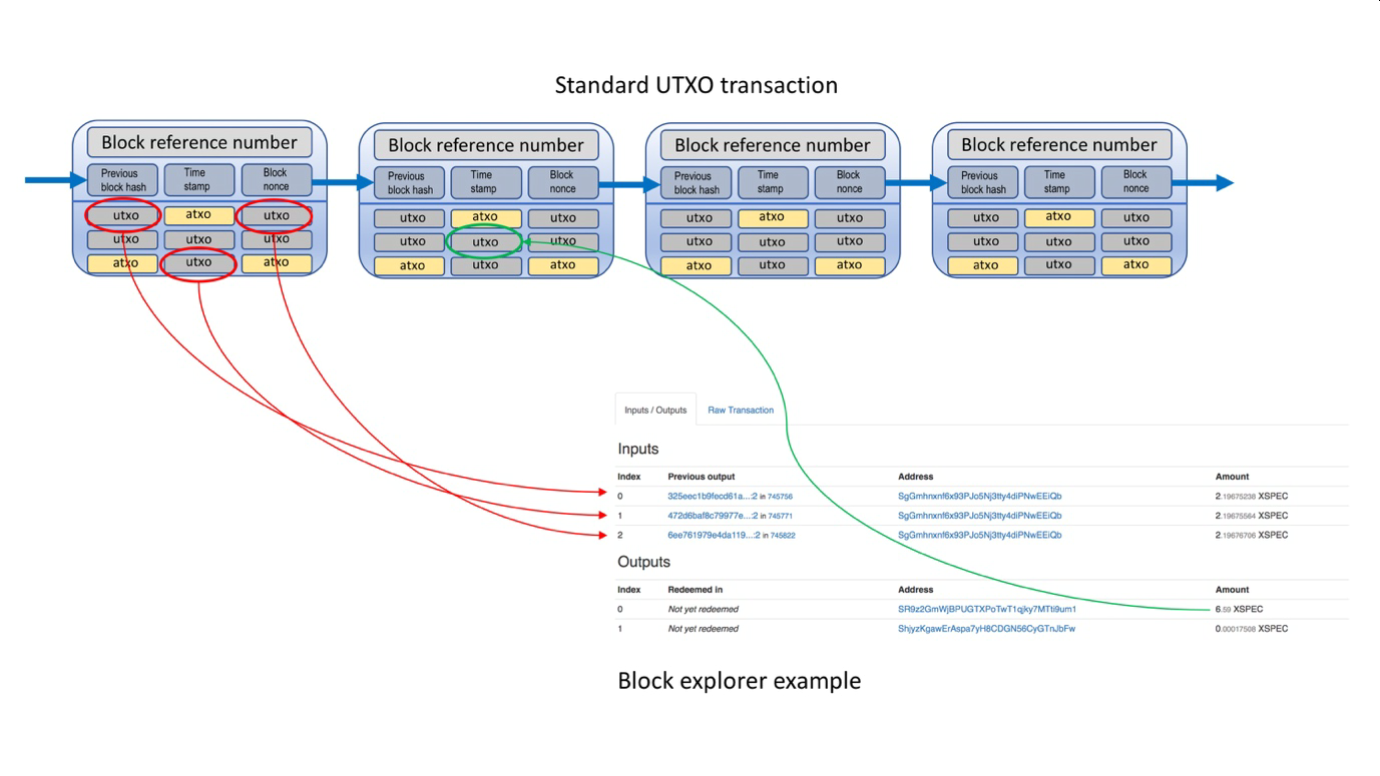
\includegraphics[width=\textwidth]{Std-UTXO-Transaction.png}
\end{figure}

On the blockchain there is a \textbf{\underline{direct}} correlation 
between the inputs and the
outputs, and all the transactions can be traced back to the genesis
transactions. This is still the case even if a mixing strategy is used,
such as in DASH. There are increasingly sophisticated methods to analyse
blockchain data and this is a growth industry. You should consider any
standard UTXO transactions to be non-anonymous and public, whether with
Spectrecoin or Bitcoin.
